\documentclass{article}
\usepackage{xeCJK} %for Chinese name
%\usepackage{helvet}
\usepackage[margin=1in]{geometry}
\usepackage{tikz}%for math trees
\setCJKmainfont{Noto Serif CJK TC}
\renewcommand{\familydefault}{\sfdefault}
\title{Introduction To Artificial Intelligence Written Assignment 1}
\author{Andr\'es Ponce(彭思安) \\
\and
0616110}
\begin{document}
\maketitle
\section{For the two videos shown in our first class(one on Robot Mouse Races, and the other one Robothespian)
, describe their respective PEAS.}
PEAS is an acronym for \textbf{P}erformance Measure, \textbf{E}nvironment, \textbf{A}ctuators, and
\textbf{S}ensors. These are 5 elements of a rational agent. A \textbf{performance measure} 
refers to the question:
How do we measure whether an agent is performing well? This will determine what factors need to be changed
for the agent to accomplish its objective. The \textbf{environment} refers to the external world in which
our object interacts(a game board, a road, etc...). The \textbf{Actuators} are the possible actions that 
our agent can perform, such as a move in a game, or turning right or left on an intersection. The sensors
are the parts of the agent that detect the external conditions and provide the information the agent uses
to make its decision.

RoboThespian is a humanoid-looking robot designed to complete multiple tasks that have some resemblance to 
human tasks. It is advertised as being able to talk and interact with other humans, and even simulate 
emotional responses. For RoboThespian, PEAS might look something like:
\begin{itemize}
	\item \textbf{Performance Measure} Since RoboThespian was designed originally to interact with others,	
			a possible perfomance measure could be a positive reaction from the people it interacts with,
			such as a laugh. 
			However, since RoboThespian can perform multiple activites (sing, act, etc...), an approach with 
			multiple performance measures for each activity might be more accurate. The first approach might	
			be more suitable if RoboThespian is interacting casually with other people rather than doing a
			specific activity.
	\item \textbf{Environment} Since RoboThespian relies on interaction, the environment would have to be 
			a place with one or more people for it to perform some actions and receive input in acoordance 
			to the rest of the model.
	\item \textbf{Actuators} Regardless of what acitivity RoboThespian is performing, some possible 
			actions for it to take might be speaking (possibly with different tone of voice and pitch,etc...),
			singing, moving its limbs, blinking, or some other physical response.
	\item \textbf{Sensors} RoboThespian could receive its input from the audience via a camera, physical 
			sensors on it's hands, or some other way to gauge the audience's response.
\end{itemize}

Robot Mouse Races, on the other hand, describe how a ``mouse", programmed in a certain way, can run through 
a maze without help and even find the best route through it.  Some of this agent's features are described below:

\begin{itemize}
	\item \textbf{Performance Measure} The performance measure could be quantified in how long the mouse takes to 
			complete the maze. 
	\item \textbf{Environment} The environment for the mouse would be a maze, the space where it receives inputs
			and makes decisions.
	\item \textbf{Actuators} The mouse would could either move forward, backward, turn left, turn right,
			or stop. 
	\item \textbf{Sensors} The sensors on the mouse would probably include some sort of camera to see what lies
			in front or to the sides. Also it might include some proximity sensor to indicate when it will
			hit a wall or when there is an open turn it can make, possibly at an intersection.
\end{itemize}

\section{In a popular English word game, the goal is to convert a given English word to another given English
word of the same length by changing one letter at a tie. Each intermediate word needs to be in a standard 
dictionary. For example, if the initial word is DOG and the destination word is CAT, the following is a possible
series of words: $DOG\rightarrow DOT\rightarrow HOT\rightarrow HAT \rightarrow CAT$. 
Now you are given this set of two-letter English words as your 
dictionary: \{AN, AM, AS, AT, AX, BE, BY, GO, HE, HI, IT, IS, IN, IF, ME, MY, NO, OF, OH, OK, ON, OR,
OX, SO, TO, UP, US, WE\}}
	\subsection{Find a solution from AT to IN using breadth-first search(BFS). When expanding a node,
		generate its children in alphabetical order. Use no repeated state checking. Give separated lists of 
		all the generated nodes and expanded nodes, both in the correct order.}
		\label{subsec:bfs}
		\textbf{Breadth-First Search} works by analyzing all the nodes a certain distance from the root
		before moving on to the next layer of nodes. In this game, since we can only change one letter of the
		word at every stage, in the first layer we will look at all the nodes that start with A (except for AT),
		and all the nodes that end with T. Our tree will resemble
		\begin{center}
		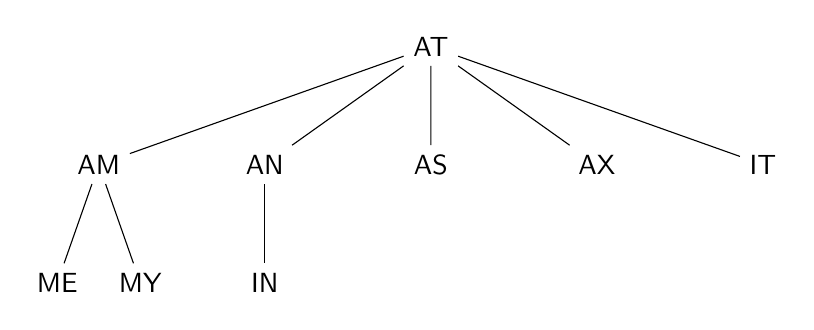
\begin{tikzpicture}[sibling distance=3em]
				\node{AT}
					child { node {AM} 
						child {node {ME}}
						child {node {MY}}
					}
					child [missing] %add empty children for spacing
					child { node {AN} 
						child{ node {IN}}
					}
					child [missing]
					child { node {AS} }
					child [missing]
					child { node {AX} }
					child [missing]
					child { node {IT} };
		\end{tikzpicture}
		\end{center}	
		The algorithm will first add into the open set all the nodes that start with A or end with T. Since 
		AM is alphabetically before AN, it will be explored first. The generated nodes will be(in the order
		they are generated): AT, AM, AS, AX, IT, ME, MY, IN.

		The fully explored nodes will be (in the order they are explored): AT, AM.
		\subsection{Explain why Hamming distance (the number of positions where the two words have 
		different letters) can be used as an admissible heuristic for this problem. You need to 
		provide a reasonable explanation.}
		\label{subsec:hamming}
		An \textbf{admissible} heuristic is one where the function $h(n)$ never overestimates the
		the true cost from the current node $n$ to the goal node. 
		
		In this problem, $h(n) \in \{0,1,2\}$, since for two letter words, the most they can differ is in their
		two letters, and will differ by none if they are the same word. We have to then show that $h(n)$ will 
		not overestimate whenever it is 0,1, or 2. 

		If $h(n) = 0$, then both of the letters in $n$ are the same as the ones in the target, which would 
		imply we reached the target and thus need to change 0 letters.
	
		If $h(n = 1)$, then the current word and the target differ by only one. In this case, the minimum amount
		of changes needed to reach the target word is 1, so $h$ will does not overestimate.

		Similar to the case where $h(n) = 1$, if $h(n = 2)$ then there are at least two words in between
		$n$ and our target, where one letter is different in each. 

		Since the true cost of the function will always be at least the Hamming distance, $h(n)$ is an 
		admissible heuristic.
	\subsection{Repeat (\ref{subsec:bfs}) using A* search with the heuristic in (\ref{subsec:hamming}).}
		The A* algorithm uses a heuristic to determine which nodes it should expand. It tries to minimize the 
		distance from the root node to the target node by finding a minimal $f(n) = g(n) + h(n)$ for every node
		it encounters. 

		At the root node AT, it will generate all its children and calculate their $f(n)$ values. The children
		will all be added to the Open set, however, AN and IT will have  $f(n) = 2$, so they will be first
		nodes to come out of the Open set at the next iteration. 

		Using A*, the generated nodes in order will be: AT, AM, AN, AS, AX, IT. The expanded nodes will be AT and 
		AN.
\section{ We have three variables X, Y, and Z. Their initial domains are digits \{0, 1,...,9\}. Given the
constraints $X = Y^{2}$ and $X=Z^{3}$, use AC-3 to update their domains to make them arc-consistent. Don't just
show the results.}

	An arc is \textbf{arc consistent} if, for a constraint $\{X_{i}, X_{j}\}$ all values of $X_{i}$ allow for
	some values of $X_{j}$. The AC-3 algorithm will take in a set of all arcs, in this problem 
	$(X, Y), (X, Z)$, check which numbers would allow the constraint to be satisfied, and discard from the 
	domains those which do not leave a possible value.

	Each of the binary constraints can be represented by two arcs, and we place all these arcs into a set,which is
	$\{(X\rightarrow Y),(Y\rightarrow X),(X\rightarrow Z),(Z\rightarrow X)\}$.
	
	When checking the first arc $(X\rightarrow Y)$, we leave in $D_{X}$ only those numbers that are squares and
	less than 10. Since our set of constraints still holds all the other arcs that involve X, we move on to the 
	next arc. For $(Y\rightarrow X)$, we leave only those numbers in Y that are perfect squares. So at this 
	point $D_{X}=[0,1,4,9]$ and $D_{Y}=[0,1,2,3]$. 

	For the third arc $(X\rightarrow Z)$, we leave in $D_{X}$ only those numbers that are also perfect cubes. 
	Since we modified $D_{X}$, we now need to add to the set of open arcs $(Y\rightarrow X)$, since now $D_{Y}$
	might need to be updated. For the arc $(Z\rightarrow X)$, we leave only those numbers who when raised 
	to the third power still exist in X. At this point $D_{X}=[0,1]$ and $D_{Z}=[0,1]$. 

	Now, we still have to re-check the arc $(Y\rightarrow X)$. Since only 0 and 1 will be in $D_{X}$ when 
	squared, $D_{Y}$ will also only contain those two numbers. 

	In the end, our three domains all contain the same numbers, namely those numbers less than 10 which are 
	perfect squares and also perfect cubes. 
	\[ D_{X} = D_{Y} = D_{Z} = [0,1]\]

\section{Consider the following cryptoarithmetic puzzle: FIVE - FOUR = ONE.}
	\subsection{Write down all the constraints. All the variables (symbols) should represent different digits.}
	The constraints in this problem would be all the relations that restrict the possible values of our symbols.
	Since $F - F = 0$, $F$ would be able to hold any value in the domain $[0-9]$. For the rest of the symbols,
	we could solve for each variable in the small equation in which they appear. For example, $I= 2O$ and 
	$O = \frac{1}{2}I$. If we write each symbol in this way, our set of constraints would be:
	\begin{center}
		\begin{tabular}{|l | r | c |}
			\hline
				F  & $[0-9]$ \\ \hline
				I  & $2O$\\ \hline
				O  & $\frac{1}{2}I$\\ \hline
				V  & $N + U$\\ \hline
				U  & $V - N$\\ \hline
				E  & $[0-9]$\\ \hline
				R  & $0$ \\ \hline
				N  & $V - U$\\ 
			\hline
		\end{tabular}	
	\end{center}
	\subsection{Solve this puzzle by hand using backtracking with forward checking and the MRV, degree, and 
	least-constraining-value heuristics. Note that the solution may not be unique.}
		\subsubsection{MRV Heuristic}
			With the \textbf{M}inimum \textbf{R}emaining \textbf{V}alues heuristic, we always choose to 
			assign the variable that has the minimum amount of legal values. Our initial values for the
			MRV heuristic, which will guide our decision, are shown in the table below.
			\begin{center}
				\begin{tabular}{|l | r | c |}
					\hline
						F  & 9 & can be any non-zero num.\\\hline
						I  & 4 & only if I/2 is also possible.\\\hline
						O  & 4 & only if 2xO is also possible.\\\hline
						V  & 7 & Non-zero, constraints also occ. 2 numbers and smallest nums.\\\hline
						U  & 7 & Non-zero, not largest, not other constraint.\\\hline
						E  & 9 & Non-zero numbers.\\\hline
						R  & 1 & Can only be zero.\\\hline
						N  & 7 & Non-zero, not largest, not other constraint.\\
					\hline
				\end{tabular}
			\end{center}
			From the formula, we can see
			that $R$ only has one posible value, since $E - R = E$  implies $R = 0$.

			For the next two variables, we have $I$ and $O$ related because $O$ is one-half of $I$, which leaves
			4 values for them to have. This means
			that $I$ has to be an even number, and $O$ has to be its half. For this, we can assign 2 to $O$ and 
			4 to $I$. 

			We now have 7 values remaining. 
			For the next couple variables, $U, V,\textrm{and } M$, they can all hold 5 values each (roughly), 
			based on the ones we have used and that two other variables have to be occupied by its constraints. 
			We know $N$ is the largest because it is constrained by a sum of the two other variables. For 
			this, we can assign a number such as 7. Now, we have to find two numbers which add to this, 
			and we can use $U=1$ and $N = 6$.

			The two variables with the greatest amounts of possible choices are $E \textrm{ and } F$. F is
			subtracted from itself and we already concluded that R is 0, so we can choose any of the remaining
			digits for these. $F = 3$ and $E = 9$ work. Since the next variable(s) to be assigned were chosen
			based on how many values we could choose from, this is an example of the MRV heuristic.
		\subsubsection{Degree}
			For the \textbf{Degree} heuristic, we have to assign the variables with the most constraints on the
			remaining variables. For this problem, we would have to start with $V, U, \textrm{ or }N$, since these
			constrain two different variables each. The amount of variables that each variable constrains
			is shown below. Again, since we are using forward checking, after each assignment we decrease the 
			domains of the other variables if applicable.
			\begin{center}
				\begin{tabular}{| l | r | c}
				\hline
				F & 0\\\hline 
				I & 1\\\hline
				O & 1\\\hline
				V & 2\\\hline
				U & 2\\\hline
				E & 1\\\hline
				R & 0\\\hline
				N & 2\\\hline
				\end{tabular}
			\end{center}
			The values with the most constraints on other variables in this problem are $V, U, \textrm{ and }N$.
			To satisfy V, we have to select only two numbers for the $U,V$ such that their sum are available 
			numbers. Since this is the earliest assignment, we can choose most of the values in the domain. We 
			can choose $5, 2, 3$ for V, U, and N, respectively. After we assign each variable, we remove it from
			the set of possible values for the unassigned variables.

			Then, we have a couple variables that only have 1 constraint. For I, we can choose a variable whose
			half is in the set of available values. We can choose $8$, since $4$ is still available. This $4$
			we can still assign to O. For $E$, we can choose any variable since E's formula allows E to be any 
			vlaue.

		Then, we have F, which has no constraints because we are subtracting it from itself, and R, which was to
		be zero by its constraint equation. We can choose 7 for F and 0 for R, respectively.
		\subsubsection{}
\end{document}

